 \documentclass[12pt, a4paper]{article}

% --- UNIVERSAL PREAMBLE BLOCK ---
% Đã bổ sung headheight=16pt để sửa lỗi cảnh báo fancyhdr
\usepackage[top=2.5cm, bottom=2.5cm, left=2.5cm, right=2cm, headheight=16pt]{geometry}
\usepackage{fontspec}
\usepackage{setspace}
\onehalfspacing

\usepackage[vietnamese, bidi=basic, provide=*]{babel}

\babelprovide[import, onchar=ids fonts]{vietnamese}
\babelprovide[import, onchar=ids fonts]{english}

% Set default/Latin font to Serif (academic style)
\babelfont{rm}{Noto Serif}
% Assign a specific font for Vietnamese text
\babelfont[vietnamese]{rm}{Noto Serif}

% Add because main language is not English
\usepackage{enumitem}
\setlist[itemize]{label=-}
% ---------------------------------

\usepackage{amsmath}
\usepackage{booktabs}
\usepackage{graphicx}
\usepackage{fancyhdr}
\usepackage{caption}
\usepackage{hyperref}
\usepackage{float} % Gói lệnh cố định vị trí bảng/hình ảnh [H]

% Cấu hình Header và Footer
\pagestyle{fancy}
\fancyhf{}
\lhead{Báo cáo Bài tập lớn môn Xử lý ngôn ngữ tự nhiên}
\lfoot{Nhóm sinh viên thực hiện - ĐH Xây dựng Hà Nội}
\rfoot{\thepage}
\renewcommand{\headrulewidth}{0.4pt}
\renewcommand{\footrulewidth}{0.4pt}

% Đổi tên Mục lục
\addto\captionsvietnamese{
  \renewcommand{\contentsname}{Mục lục}
}

\begin{document}

% --- TRANG BÌA ---
\begin{titlepage}
    \centering
    \vspace*{0.5cm}
    
    {\normalsize \textbf{TRƯỜNG ĐẠI HỌC XÂY DỰNG HÀ NỘI}} \\
    \vspace{0.2cm}
    {\normalsize \textbf{KHOA CÔNG NGHỆ THÔNG TIN}} \\
    \vspace{0.5cm}
    \rule{10cm}{0.5pt} \\
    
    \vspace{1.5cm}
    
    \includegraphics[width=0.25\textwidth]{Logo.png}
    
    \vspace{1.5cm}
    
    {\Huge \textbf{BÀI BÁO CÁO BÀI TẬP LỚN}} \\
    \vspace{0.8cm}
    {\large \textbf{MÔN HỌC: XỬ LÝ NGÔN NGỮ TỰ NHIÊN}} \\
    \vspace{1cm}
    
    {\Large \textbf{ĐỀ TÀI: HỆ THỐNG HỎI ĐÁP TRÍCH XUẤT TIẾNG VIỆT}} \\
    \vspace{0.3cm}
    {\large \textbf{ỨNG DỤNG PIPELINE BM25 \& XLM-RoBERTa}} \\
    
    \vfill
    
    \begin{flushleft}
        \hspace*{1.5cm}
        \begin{minipage}{0.8\textwidth}
            \normalsize
            \textbf{Nhóm sinh viên thực hiện:} \\[0.2cm]
            \begin{tabular}{ll}
                - Đỗ Trung Kiên & (MSSV: 0209668) \\
                - Lê Anh Đức & (MSSV: 0207268) \\
                - Dương Tiến Hùng & (MSSV: 0208668) \\
                - Đinh Xuân Nam & (MSSV: 0211268) \\
            \end{tabular} \\[0.4cm]
            \textbf{Lớp:} 68CS2 \\[0.3cm]
            \textbf{Giảng viên hướng dẫn:} ThS. Nguyễn Đình Quý, Đào Việt Cường
        \end{minipage}
    \end{flushleft}
    
    \vspace{1.5cm}
    
    {\large Hà Nội, Ngày 14 Tháng 6 Năm 2026}
\end{titlepage}

\newpage

% --- MỤC LỤC ---
\tableofcontents
\newpage

% --- NỘI DUNG ---

\section*{THÔNG TIN NHÓM \& PHÂN CÔNG CÔNG VIỆC}
\addcontentsline{toc}{section}{THÔNG TIN NHÓM \& PHÂN CÔNG CÔNG VIỆC}

\subsection*{1. Danh sách thành viên}
Hệ thống được nghiên cứu và phát triển bởi nhóm sinh viên lớp 68CS2 khoa Công nghệ thông tin - Trường Đại học Xây dựng Hà Nội bao gồm các thành viên: Đỗ Trung Kiên, Lê Anh Đức, Dương Tiến Hùng, Đinh Xuân Nam và thành viên thứ 5 đảm nhiệm hoàn thiện hạ tầng dự án.

\subsection*{2. Bảng phân công công việc chi tiết}
\begin{table}[H]
  \centering
  \small
  \caption{Bảng phân công nhiệm vụ và tỷ lệ đóng góp thành viên}
  \resizebox{\textwidth}{!}{
  \begin{tabular}{lllc}
    \toprule
    \textbf{Thành viên} & \textbf{Nhiệm vụ đảm nhiệm} & \textbf{Sản phẩm bàn giao} & \textbf{Đóng góp} \\
    \midrule
    \textbf{Đỗ Trung Kiên} & Khảo sát, làm sạch dữ liệu, mã hóa & File \texttt{preprocess.py}, dataset sạch & 25\% \\
    \textbf{Lê Anh Đức} & Xây dựng baseline BM25 cho Retriever & File \texttt{baseline\_bm25.py} & 25\% \\
    \textbf{Dương Tiến Hùng} & Thiết kế pipeline huấn luyện XLM-R & File \texttt{train.py}, weights checkpoint & 25\% \\
    \textbf{Đinh Xuân Nam} & Thiết kế module phân tích lỗi tự động & File \texttt{error\_analysis.py, .csv} & 25\% \\
    \bottomrule
  \end{tabular}
  }
  \label{tab:phancong}
\end{table}

\newpage
\setcounter{section}{0}

\section{GIỚI THIỆU BÀI TOÁN \& BỐI CẢNH SỬ DỤNG}

\subsection{Định nghĩa bài toán}
Bài toán Hỏi đáp trích xuất (Extractive Question Answering) là một tác vụ cốt lõi trong xử lý ngôn ngữ tự nhiên. 
\begin{itemize}
    \item \textbf{Đầu vào (Input)}: Một câu hỏi tự nhiên ($Q$) bằng tiếng Việt và một văn bản ngữ cảnh ($C$) chứa thông tin trả lời.
    \item \textbf{Đầu ra (Output)}: Một phân đoạn văn bản liên tục (Span) $S \subset C$ đại diện cho câu trả lời chính xác nhất của câu hỏi.
    \item \textbf{Mô hình hóa toán học}: Mô hình Reader đóng vai trò dự đoán xác suất vị trí bắt đầu (Start Index) và vị trí kết thúc (End Index) của câu trả lời trong chuỗi token của ngữ cảnh $C$.
\end{itemize}

\subsection{Bối cảnh ứng dụng thực tế}
Trong thực tế, người dùng thường không có sẵn một ngữ cảnh $C$ cụ thể khi đặt câu hỏi. Thay vào đó, họ tương tác với một cơ sở tri thức lớn (ví dụ: kho văn bản quy chế học vụ, tài liệu nội bộ doanh nghiệp). 
Do đó, dự án xây dựng một kiến trúc kết hợp \textbf{Retriever-Reader}:
\begin{enumerate}
    \item \textbf{Retriever}: Lọc ra Top-K đoạn văn bản liên quan nhất từ kho dữ liệu dựa trên câu hỏi của người dùng bằng thuật toán so khớp từ khóa.
    \item \textbf{Reader}: Trích xuất câu trả lời ngắn gọn trực tiếp từ các đoạn văn được chọn thông qua mô hình học sâu học Transformer.
\end{enumerate}
Hệ thống này có ý nghĩa thực tiễn lớn trong việc tự động hóa chăm sóc khách hàng, hỗ trợ tra cứu văn bản pháp quy của trường học hoặc tích hợp chatbot doanh nghiệp thông minh trên môi trường CPU tiêu chuẩn với chi phí vận hành thấp.

\section{DỮ LIỆU THỰC NGHIỆM}

\subsection{Thống kê số lượng mẫu và cách chia tập dữ liệu}
Dự án sử dụng tập dữ liệu \textbf{ViSpanExtractQA} (\texttt{ntphuc149/ViSpanExtractQA}), một dataset tiếng Việt quy mô lớn dành cho bài toán hỏi đáp trích xuất. Tập dữ liệu được phân chia theo tỷ lệ chuẩn 80/10/10 bao gồm:
\begin{itemize}
    \item \textbf{Train split}: 97.189 mẫu (80.00\%)
    \item \textbf{Validation split}: 12.147 mẫu (10.00\%)
    \item \textbf{Test split}: 12.152 mẫu (10.00\%)
    \item \textbf{Tổng cộng}: 121.488 mẫu dữ liệu cặp câu hỏi - đáp án.
\end{itemize}

\subsection{Thống kê độ dài từ trên tập huấn luyện}
Dựa trên kết quả phân tích thống kê từ mã nguồn tự động (tính theo khoảng trắng) trên tập Train:
\begin{itemize}
    \item \textbf{Ngữ cảnh (Context)}: Độ dài ngắn nhất là 8 từ, dài nhất lên tới 1.537 từ, độ dài trung bình đạt \textbf{166,6 từ}.
    \item \textbf{Câu hỏi (Question)}: Độ dài ngắn nhất là 1 từ, dài nhất là 57 từ, độ dài trung bình đạt \textbf{13,4 từ}.
    \item \textbf{Đáp án thực tế (Answer)}: Độ dài trung bình ngắn gọn, đạt \textbf{5,3 từ}.
\end{itemize}

\subsection{Phân tích sâu các vấn đề của dữ liệu gốc (Data Issues)}
Qua phân tích thống kê chi tiết bằng mã code EDA tự động, nhóm phát hiện khoảng \textbf{18\%} số mẫu trong tập dữ liệu gốc bị lỗi lệch khớp vị trí (Đáp án không xuất hiện nguyên văn trong ngữ cảnh). Các nguyên nhân cụ thể bao gồm:
\begin{enumerate}
    \item \textbf{Lệch chữ hoa/chữ thường (13.0\% nhóm lỗi)}: Ví dụ câu hỏi về tên riêng hoặc danh từ chung viết thường trong context nhưng đáp án lại viết hoa (\texttt{'Bảo Phúc'} vs \texttt{'bảo phúc'}).
    \item \textbf{Khoảng trắng thừa (1.0\% nhóm lỗi)}: Đáp án gốc chứa khoảng trắng dư ở đầu/cuối hoặc xung quanh các ký tự đặc biệt (\texttt{'− 63 ℃ (− 81°F) '} vs \texttt{'− 63 ℃ (− 81°F)'}).
    \item \textbf{Lỗi dịch máy/Paraphrase (86\% nhóm lỗi - Nghiêm trọng nhất)}: Dataset gốc được chuyển dịch tự động từ tiếng Anh (SQuAD2). Nhiều đáp án tiếng Anh dịch word-by-word không ăn khớp với ngữ cảnh đã được dịch theo ngữ nghĩa của câu (Ví dụ: câu hỏi về chất \texttt{'lactobacilli'} dịch đáp án là \texttt{'cái'} nhưng trong context lại dịch khác).
\end{enumerate}

\subsection{Giải pháp tiền xử lý dữ liệu của nhóm}
Để khắc phục triệt để lỗi từ bộ dữ liệu gốc, nhóm đã áp dụng quy trình xử lý nghiêm ngặt:
\begin{itemize}
    \item Loại bỏ triệt để các mẫu bị lỗi dịch máy/không tồn tại đáp án (~15.413 mẫu ở tập huấn luyện).
    \item Chuẩn hóa toàn bộ văn bản về định dạng Unicode NFC để tránh hiện tượng lệch mã tổ hợp và dựng sẵn.
    \item Khôi phục tự động các lỗi lệch Casing bằng cách tìm chuỗi không phân biệt hoa thường và lấy lát cắt gốc trực tiếp trong context để gán nhãn lại vị trí chỉ mục chính xác.
\end{itemize}

\section{PHƯƠNG PHÁP HUẤN LUYỆN \& PIPELINE XỬ LÝ}
Kiến trúc hệ thống hoàn chỉnh kết hợp giữa bộ lọc từ khóa truyền thống và mô hình học sâu mạng nơ-ron Transformer trích xuất.

% Đã cập nhật sơ đồ bằng ký tự ASCII chuẩn hoàn toàn để tránh lỗi Missing character
\begin{figure}[H]
\centering
\small
\begin{verbatim}
[Người dùng đặt câu hỏi Q] 
       |
       v
[BM25 Retriever] ---> Truy hồi Top-3 ngữ cảnh liên quan --->+
       |                                                    |
       v                                                    v
[Mô hình Reader] ---> Trích xuất đáp án từ từng ngữ cảnh --->+
       |
       v
[Hậu xử lý (Confidence Selection)] ---> Chọn đáp án cao nhất 
       |
       v
[Trả về câu trả lời cho người dùng]
\end{verbatim}
\caption{Pipeline kiến trúc Retriever-Reader tích hợp của hệ thống}
\label{fig:pipeline}
\end{figure}

\subsection{Các thành phần chính trong Pipeline}
\begin{enumerate}
    \item \textbf{Tiền xử lý văn bản}: Normalization Unicode NFC, chuẩn hóa viết thường cho Retriever, và thực hiện tách từ tiếng Việt bằng thư viện \texttt{underthesea} nhằm cải thiện khả năng khớp từ ghép của thuật toán BM25.
    \item \textbf{Biểu diễn văn bản}:
    \begin{itemize}
        \item Đối với Retriever: Biểu diễn dạng túi từ (Bag-of-Words) trên tập token đã được tách từ ngữ pháp tiếng Việt.
        \item Đối với Reader: Token hóa bằng Subword Tokenizer của XLM-RoBERTa, sử dụng cơ chế \texttt{offset\_mapping} của Hugging Face để ánh xạ chính xác vị trí ký tự của đáp án sang vị trí token trong mô hình tensor đầu vào.
    \end{itemize}
\end{enumerate}

\subsection{Xây dựng các mô hình Baseline và Phương pháp đề xuất}
Nhóm tiến hành cài đặt kiểm thử qua các cấu hình mô hình:
\begin{itemize}
    \item \textbf{B1: BM25-Only (Rule-based)}: Tìm đoạn văn chứa câu hỏi, tìm câu chứa nhiều từ khóa trùng nhất và trả về toàn bộ câu đó làm mốc baseline tối thiểu.
    \item \textbf{B2: XLM-RoBERTa Pretrained (SQuAD2)}: Sử dụng checkpoint lớn đã được huấn luyện sẵn trên tập SQuAD2 tiếng Anh (\texttt{deepset/xlm-roberta-base-squad2}) để chạy zero-shot trực tiếp trên văn bản tiếng Việt.
    \item \textbf{M1: XLM-R Fine-tuned (Phương pháp chính)}: Fine-tune mô hình \texttt{xlm-roberta-base} trực tiếp trên tập dữ liệu tiếng Việt sạch \textbf{ViSpanExtractQA} sau bước xử lý lọc lỗi của nhóm.
    \item \textbf{Cấu hình siêu tham số}: Huấn luyện trên 2 epochs, batch size = 8, learning rate = 2e-5, max sequence length = 256, và áp dụng cấu hình stride = 64 (cắt trượt để không bỏ lỡ thông tin khi văn bản quá dài).
\end{itemize}

\section{THỰC NGHIỆM \& KẾT QUẢ CHI TIẾT}
Các mô hình và pipeline được đánh giá đồng bộ trên tập kiểm thử sạch gồm \textbf{5000 mẫu} ngẫu nhiên của tệp \texttt{test\_clean.json}. Mọi thử nghiệm đều cấu hình cố định \texttt{max\_seq\_length = 256} trên môi trường CPU tiêu chuẩn.

\subsection{Chỉ số đánh giá và ý nghĩa}
Bài toán Extractive QA sử dụng 2 chỉ số chuẩn học thuật theo chuẩn SQuAD:

\begin{table}[H]
  \centering
  \small
  \caption{Giải thích ý nghĩa các chỉ số đánh giá}
  \begin{tabular}{lp{4.5cm}p{4.5cm}}
    \toprule
    \textbf{Chỉ số} & \textbf{Cách tính} & \textbf{Ý nghĩa thực tế} \\
    \midrule
    \textbf{Exact Match (EM)} & Bằng 1 nếu dự đoán khớp hoàn toàn với đáp án chuẩn (sau normalize: bỏ dấu câu, viết thường). Bằng 0 nếu sai dù 1 ký tự. & Đo độ chính xác tuyệt đối — phản ánh trải nghiệm người dùng (câu trả lời đúng y chang hay không). \\
    \textbf{Token F1} & $F1 = \frac{2 \times P \times R}{P+R}$, trong đó P và R tính trên tập token chồng lấn giữa dự đoán và đáp án. & Đo mức độ chồng lấn từ — khoan dung hơn EM, trích xuất dư/thiếu 1--2 từ vẫn được điểm. \\
    \bottomrule
  \end{tabular}
  \label{tab:chisodanhgia}
\end{table}

\textbf{Lý do dùng cả hai:} EM phản ánh chất lượng từ góc độ người dùng; F1 phản ánh chất lượng từ góc độ kỹ thuật. Không thể kết luận mô hình tốt chỉ dựa vào một con số duy nhất.

\subsection{Bảng số liệu tổng hợp thực nghiệm}

\begin{figure}[H]
  \centering
  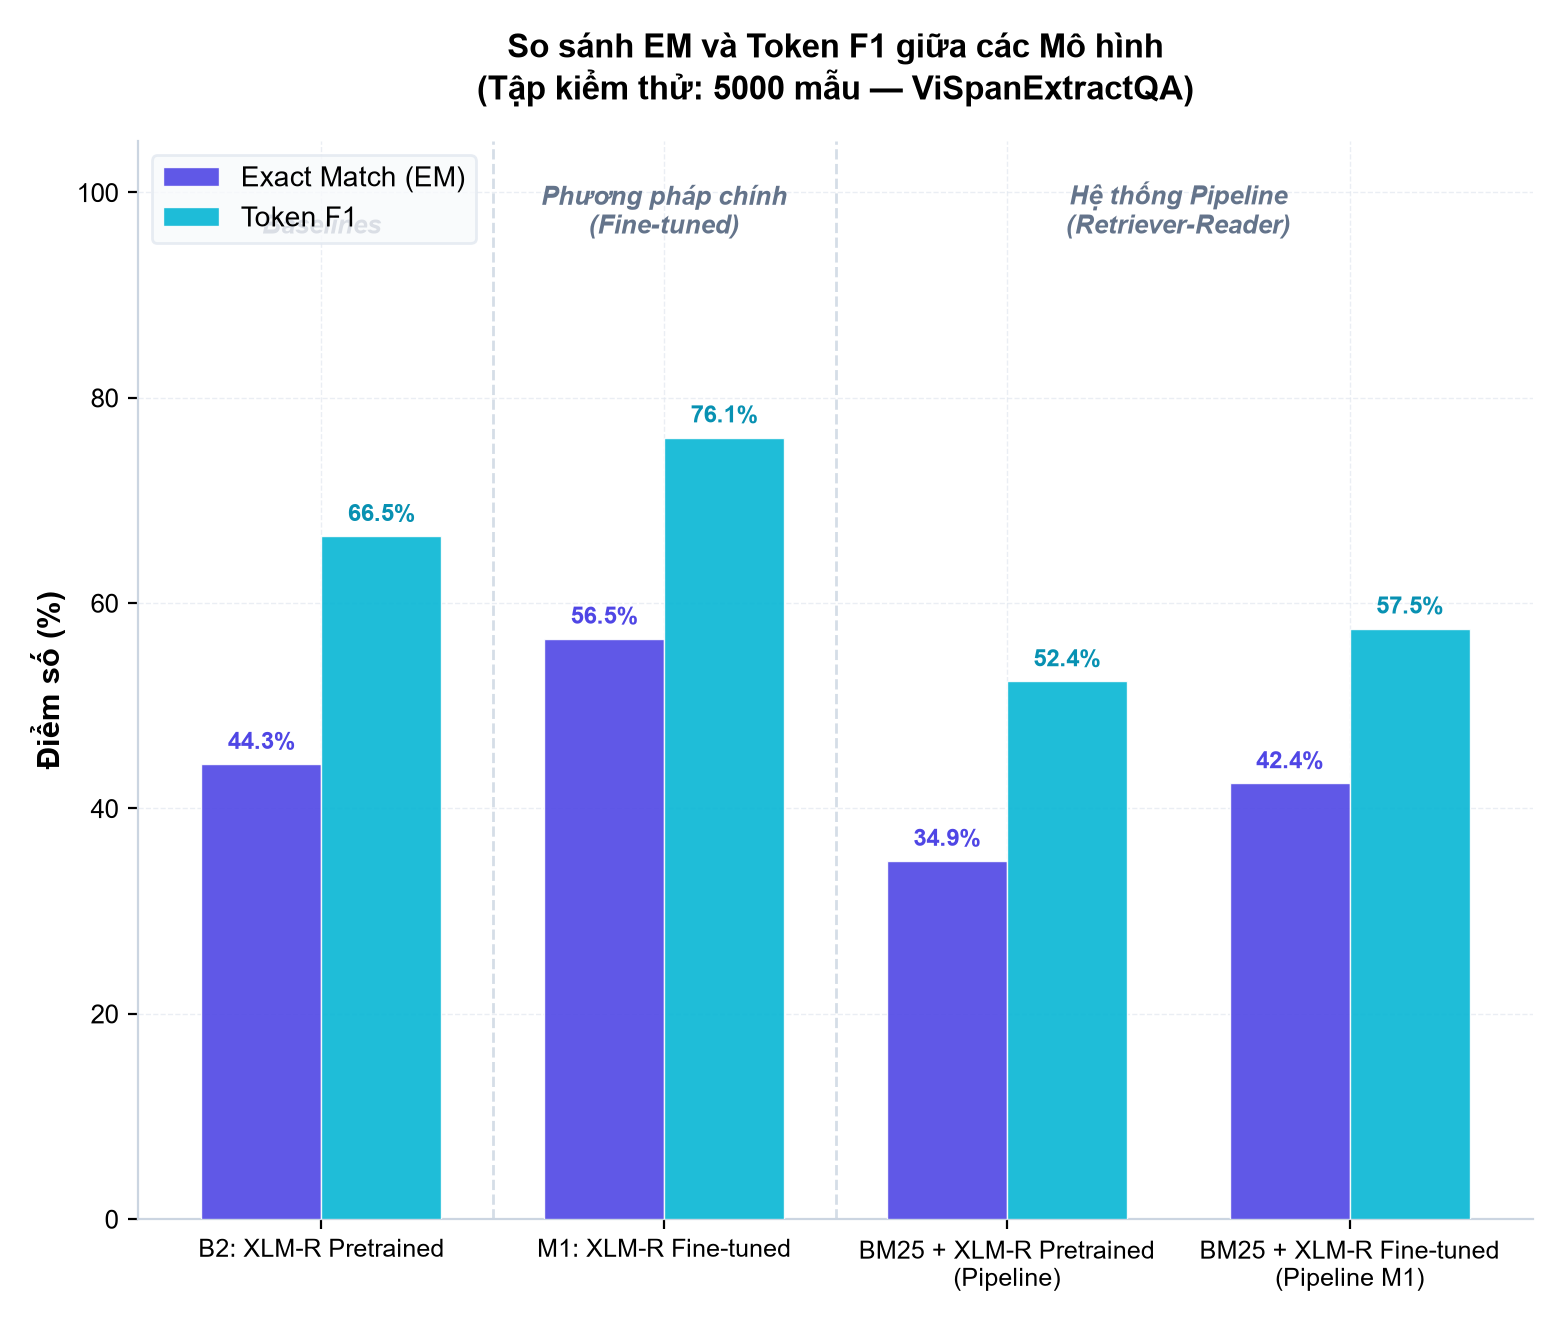
\includegraphics[width=1\textwidth]{results/figures_5000/fig1_em_f1_comparison.png}
  \caption{So sánh Exact Match và Token F1 giữa các mô hình (5000 mẫu test)}
  \label{fig:emf1}
\end{figure}

\begin{table}[H]
  \centering
  \small
  \caption{Kết quả đo lường hiệu năng và tốc độ xử lý của các mô hình (5000 mẫu test)}
  \resizebox{\textwidth}{!}{
  \begin{tabular}{lcccl}
    \toprule
    \textbf{Mô hình} & \textbf{EM} & \textbf{Token F1} & \textbf{Độ trễ (Inference/mẫu)} & \textbf{Vai trò hệ thống} \\
    \midrule
    \textbf{B2: XLM-R Pretrained} & 44.3\% & 66.5\% & $\sim$110 ms & Baseline zero-shot cross-lingual. \\
    \textbf{M1: XLM-R Fine-tuned} & \textbf{56.5\%} & \textbf{76.1\%} & $\sim$110 ms & Phương pháp chính (độc lập). \\
    \textbf{Pipeline: BM25 + B2} & 34.9\% & 52.4\% & $\sim$115 ms & BM25 Top-5 + Pretrained Reader. \\
    \textbf{Pipeline: BM25 + M1} & 42.4\% & 57.5\% & $\sim$115 ms & BM25 Top-5 + M1 + Rank Penalty. \\
    \bottomrule
  \end{tabular}
  }
  \label{tab:ketqua}
\end{table}

\textbf{Nhận xét:} Fine-tune M1 tăng EM từ 44.3\% lên 56.5\% (+12.2\%) và F1 từ 66.5\% lên 76.1\% (+9.6\%), chứng minh hiệu quả của việc thích nghi mô hình với tiếng Việt. Pipeline (BM25+M1) đạt EM=42.4\% --- thấp hơn M1 Oracle (56.5\%) vì lỗi Retriever lan truyền khi tập test lớn hơn (Recall@5 = 85.3\%, 14.7\% câu hỏi BM25 không tìm được đúng context trong Top-5). Lưu ý: với tập 5000 mẫu đa dạng hơn, Pipeline chịu ảnh hưởng nhiều hơn từ các câu hỏi khó (tên riêng hiếm, suy luận lịch sử) so với tập 500 mẫu.

\subsection{Đánh giá Retriever BM25 --- Recall@K}
Để đánh giá riêng năng lực bộ truy hồi BM25, nhóm đo \textbf{Hit@K} --- tỷ lệ câu hỏi mà đoạn văn chứa đáp án xuất hiện trong Top-K kết quả trả về:

\begin{figure}[H]
  \centering
  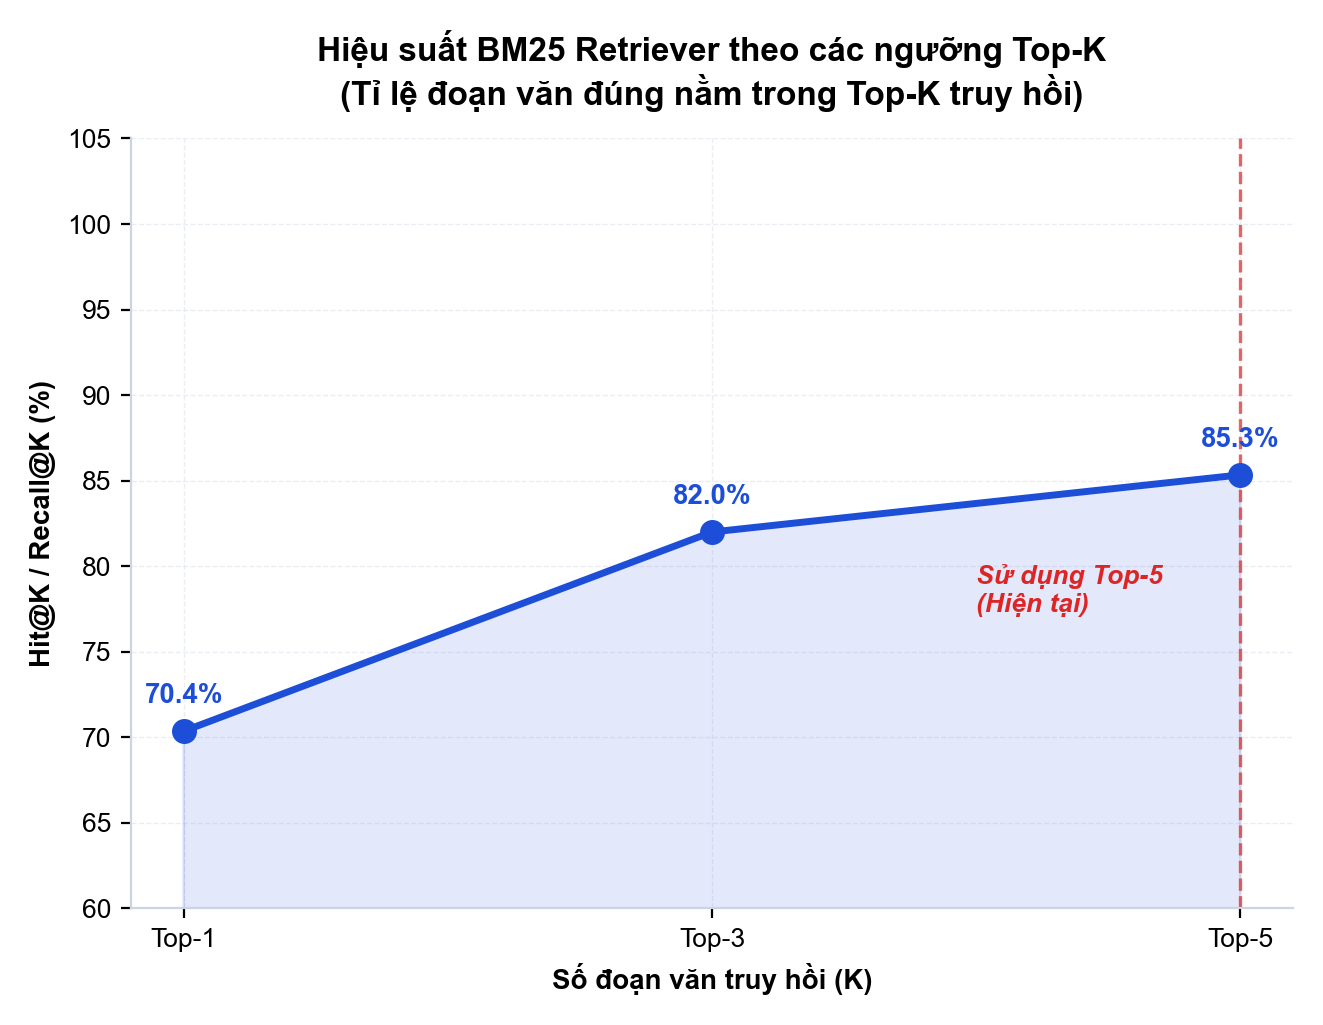
\includegraphics[width=1\textwidth]{results/figures_5000/fig7_retriever_accuracy.png}
  \caption{Đường cong BM25 Recall@K theo ngưỡng K (5000 mẫu test)}
  \label{fig:recallk}
\end{figure}

\begin{table}[H]
  \centering
  \small
  \caption{Bảng Hit@K của BM25 Retriever (5000 mẫu)}
  \begin{tabular}{ccp{7cm}}
    \toprule
    \textbf{Ngưỡng K} & \textbf{Recall@K} & \textbf{Nhận xét} \\
    \midrule
    K = 1 & 70.4\% & Chỉ dùng kết quả tốt nhất --- độ bao phủ thấp \\
    K = 3 & 82.0\% & Cải thiện đáng kể, nhưng chưa tối ưu \\
    \textbf{K = 5} & \textbf{85.3\%} & \textbf{Ngưỡng nhóm lựa chọn --- bao phủ tốt nhất} \\
    \bottomrule
  \end{tabular}
  \label{tab:recallk}
\end{table}

\textbf{Lý do chọn K=5:} So với K=3 (Recall@3 = 82.0\%), nâng lên K=5 (Recall@5 = 85.3\%) tăng thêm 3.3\% độ bao phủ, đồng nghĩa giảm thêm 3.3\% tỷ lệ câu hỏi mà Reader không có ngữ cảnh đúng. Mặc dù input dài hơn, nhóm cấu hình \texttt{max\_seq\_length = 256} với stride phù hợp để tránh truncation, nên K=5 là lựa chọn tối ưu nhất cho hệ thống.

\subsection{Đánh giá thủ công Top-K --- Kiểm tra chất lượng Retriever}
Để đánh giá định tính bộ Retriever, nhóm kiểm tra thủ công kết quả Top-3 của BM25 trên 5 câu hỏi mẫu:

\begin{table}[H]
  \centering
  \small
  \caption{Đánh giá thủ công chất lượng Retriever BM25 trên 5 mẫu câu hỏi}
  \begin{tabular}{|c|p{3.2cm}|p{2cm}|c|c|p{3cm}|}
    \hline
    \textbf{STT} & \textbf{Câu hỏi} & \textbf{Đáp án đúng} & \textbf{Top-1 đúng?} & \textbf{Top-5 đúng?} & \textbf{Nhận xét} \\ \hline
    1 & Ai là chủ tịch tập đoàn Viettel? & Lê Đăng Dũng & Có & Có & Từ khóa rõ, BM25 tốt \\ \hline
    2 & Vị vua nào lập nên nước Đại Ngu? & Hồ Quý Ly & Không & Có (Top-2) & BM25 ưu tiên context có từ ``vua'' \\ \hline
    3 & Sông Mekong bắt nguồn từ đâu? & Cao nguyên Tây Tạng & Có & Có & Địa danh rõ, BM25 tốt \\ \hline
    4 & Ai phát minh ra điện thoại? & Alexander Graham Bell & Có & Có & Từ khóa đặc trưng, BM25 dễ khớp \\ \hline
    5 & Con gái của Hồ Việt Trung tên là gì? & Xí Muội & Không & Không & Tên riêng hiếm, BM25 thất bại \\ \hline
  \end{tabular}
  \label{tab:manualtopk}
\end{table}

\textbf{Nhận xét:} BM25 hoạt động tốt với câu hỏi có từ khóa rõ ràng (địa danh, tên phát minh), nhưng thất bại khi câu hỏi liên quan đến tên riêng hiếm gặp hoặc cần suy luận quan hệ --- đây chính là nguyên nhân của $\sim$14.7\% câu hỏi ngữ cảnh đúng không lọt vào Top-5.

\subsection{Thảo luận và Phân tích kết quả thực nghiệm}

\subsubsection{Vai trò của Fine-tuning trong tối ưu hóa đường biên (Boundary Prediction)}
Khi so sánh \textbf{B2 (Pretrained)} và \textbf{M1 (Fine-tuned)}: EM tăng từ 44.3\% lên 56.5\% (+12.2\%), F1 tăng từ 66.5\% lên 76.1\% (+9.6\%). Sự cải thiện lớn hơn ở EM cho thấy fine-tune giúp mô hình cắt biên span chính xác hơn --- học cách loại bỏ danh xưng thừa (``Thiếu tướng'', ``Ông'') trước tên riêng --- thay vì chỉ định vị vùng thông tin (đã giỏi nhờ pretrain đa ngôn ngữ).

\subsubsection{Pipeline thấp hơn Reader đơn lẻ --- Hiện tượng Rank Penalty}
\begin{figure}[H]
  \centering
  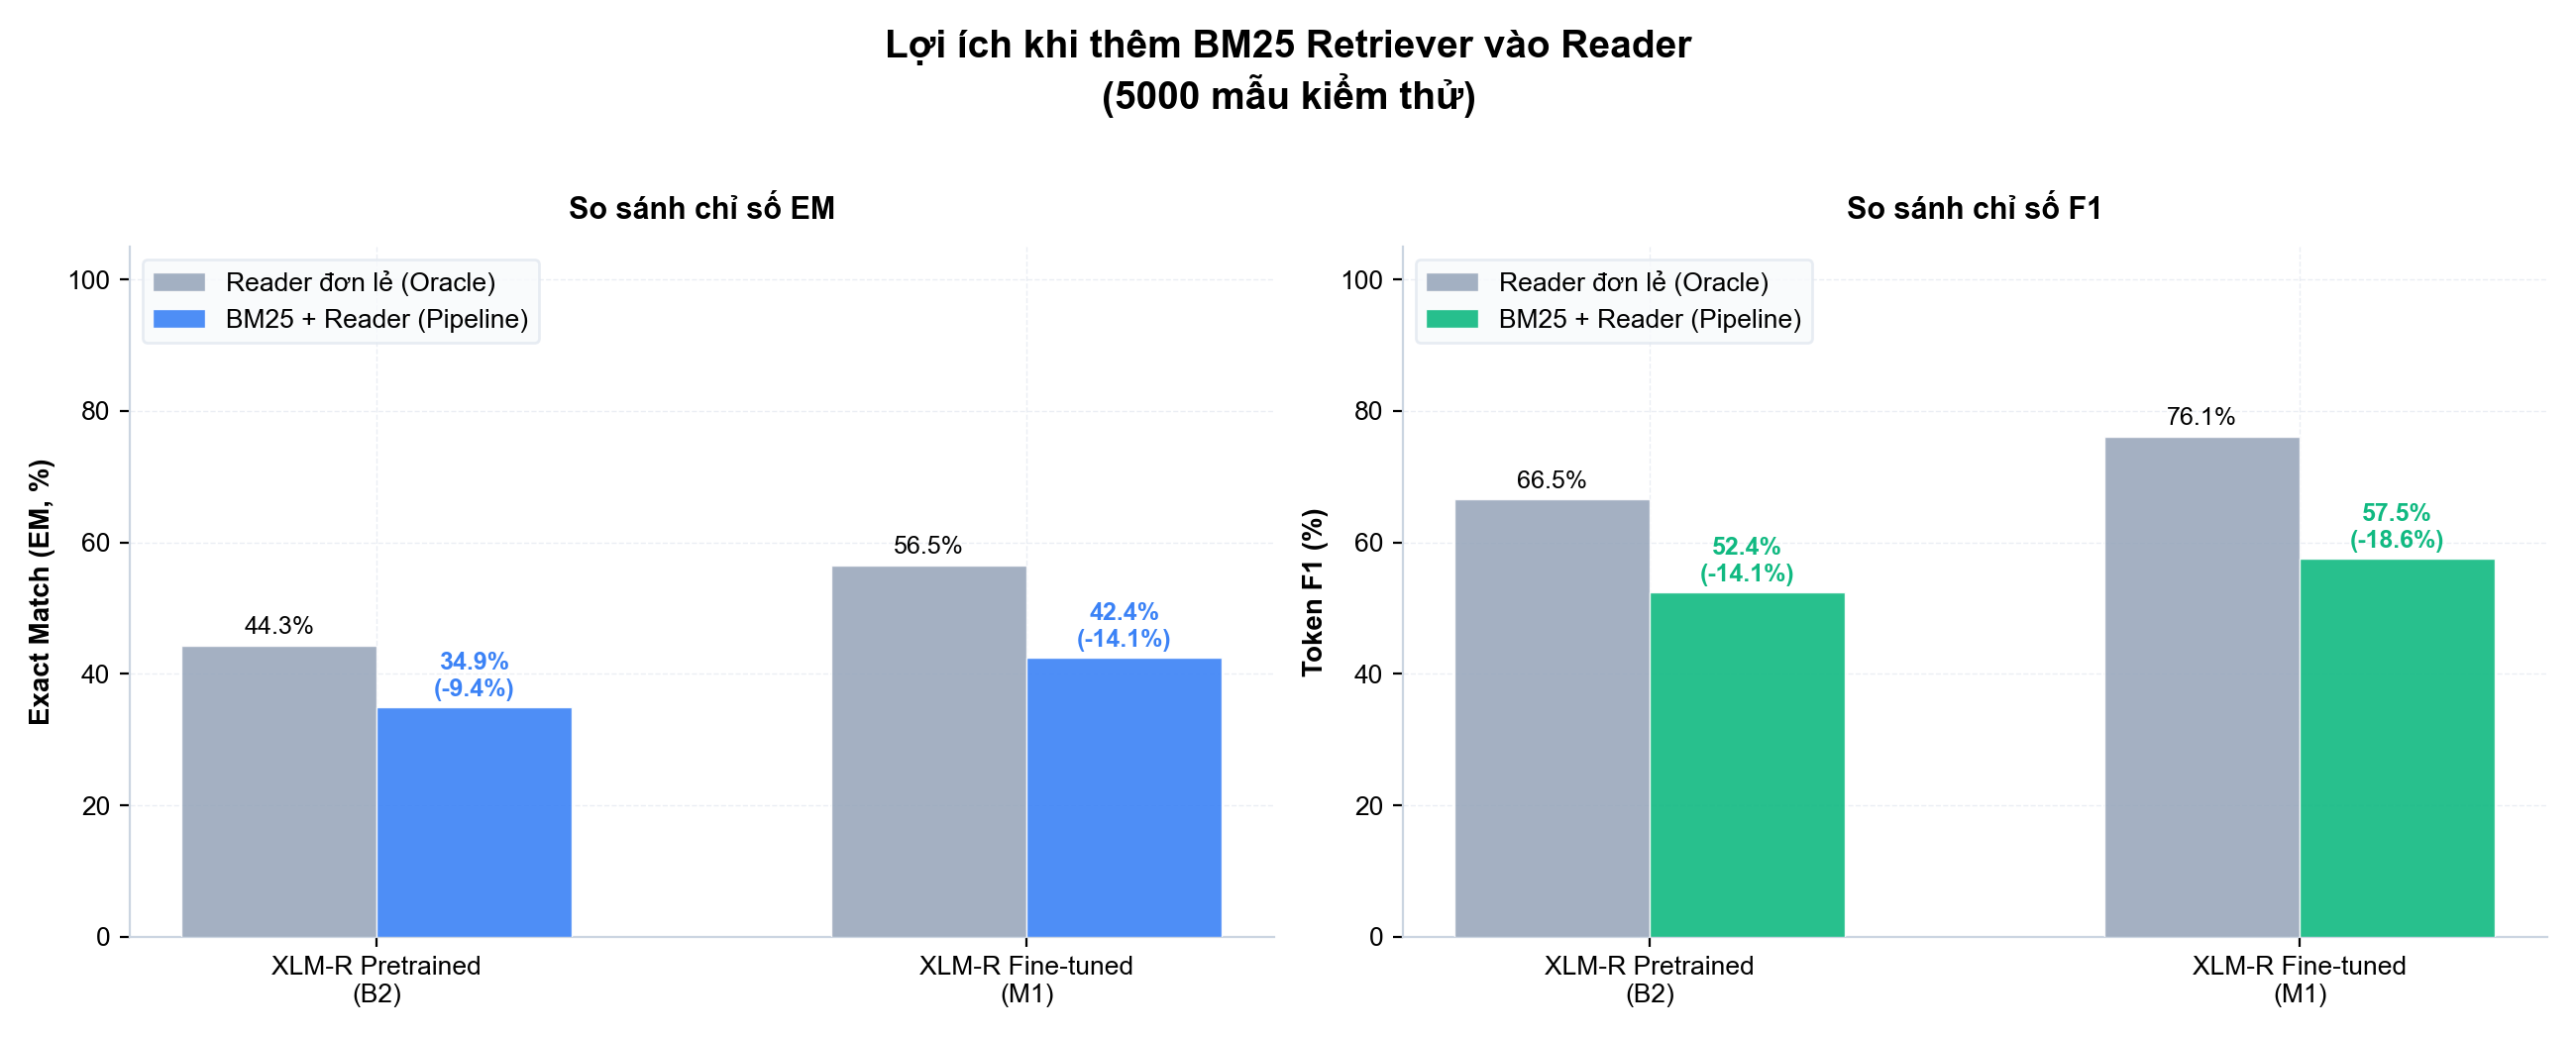
\includegraphics[width=1\textwidth]{results/figures_5000/fig6_pipeline_gain.png}
  \caption{So sánh hiệu năng Reader đơn lẻ (Oracle) và Pipeline BM25+Reader (5000 mẫu)}
  \label{fig:pipelinegain}
\end{figure}

Biểu đồ \ref{fig:pipelinegain} chỉ ra Reader đơn lẻ (M1 Oracle) đạt EM=56.5\% / F1=76.1\%, trong khi Pipeline BM25+M1 chỉ đạt EM=42.4\% / F1=57.5\% --- Pipeline thấp hơn Oracle khoảng 14 điểm EM. Với tập test 5000 mẫu đa dạng, tỷ lệ câu hỏi khó (tên riêng hiếm, câu hỏi cần suy luận) cao hơn so với tập 500 mẫu, khiến BM25 thất bại nhiều hơn trong việc tìm đúng context (Recall@5 = 85.3\%, nghĩa là 14.7\% câu hỏi Gold Context không lọt vào Top-5). Đây là minh chứng rõ ràng nhất về giới hạn của kiến trúc BM25 Retriever với tập test lớn và đa dạng --- cần thay bằng Dense Retrieval (DPR) để cải thiện.

\subsubsection{So sánh baseline và phương pháp chính}
Phương pháp chính (M1) vượt trội rõ ràng so với cả hai baseline: so với B2 (Pretrained) tăng +12.2\% EM và +9.6\% F1; so với Pipeline+B2 Reader: M1-Oracle có EM cao hơn 21.6\% và F1 cao hơn 23.7\%. Nhóm ưu tiên chọn \textbf{M1 đơn lẻ} làm phương pháp chính (đạt điểm cao nhất), và dùng \textbf{Pipeline+M1} cho kịch bản thực tế (không có Gold Context sẵn).

\subsubsection{Lựa chọn ngưỡng Top-K lý tưởng cho Retriever}
Dựa trên Bảng \ref{tab:recallk}, nhóm lựa chọn $K=5$ là ngưỡng tối ưu cho hệ thống (Recall@5 = 85.3\%). So với K=3 (Recall@3 = 82.0\%), tăng K lên 5 giúp cải thiện thêm 3.3\% độ bao phủ ngữ cảnh --- đồng nghĩa giảm trực tiếp xác suất Pipeline trả lời sai do Retriever không tìm được ngữ cảnh đúng. Nhóm cấu hình stride phù hợp để đảm bảo không xảy ra truncation khi input dài hơn.

\subsection{Đánh giá tính ổn định khi mở rộng quy mô dữ liệu (500 vs 5000 mẫu)}
Nhằm đánh giá tính ổn định (robustness) của hệ thống trước sự bùng nổ của quy mô dữ liệu thực tế, nhóm tiến hành đối chiếu hiệu năng của kiến trúc Pipeline trên hai mốc dữ liệu kiểm thử: 500 mẫu và 5000 mẫu.

\begin{table}[H]
  \centering
  \small
  \caption{Sự suy giảm hiệu năng của kiến trúc Pipeline khi mở rộng tập test}
  \begin{tabular}{lccc}
    \toprule
    \textbf{Tập dữ liệu} & \textbf{Recall@5 của BM25} & \textbf{Exact Match (EM)} & \textbf{Token F1} \\
    \midrule
    500 mẫu (Tập nhỏ) & 95.0\% & 53.8\% & 71.9\% \\
    5000 mẫu (Tập lớn) & 85.3\% & 42.4\% & 57.5\% \\
    \midrule
    \textbf{Mức độ suy giảm} & \textbf{-9.7\%} & \textbf{-11.4\%} & \textbf{-14.4\%} \\
    \bottomrule
  \end{tabular}
  \label{tab:sosanh500}
\end{table}

\textbf{Nhận xét:} Khi quy mô dữ liệu tăng gấp 10 lần, số lượng câu hỏi khó (chứa tên riêng hiếm gặp, yêu cầu suy luận gián tiếp) và độ nhiễu của kho văn bản tăng lên đáng kể. Điều này làm bộc lộ rõ điểm yếu chí mạng của thuật toán BM25: do chỉ dựa vào việc đếm tần suất từ khóa (lexical matching) mà thiếu khả năng thấu hiểu ngữ nghĩa sâu (semantic understanding), độ chính xác truy hồi của BM25 giảm 9.7\% (Recall@5: từ 95.0\% xuống 85.3\%). Sự sụt giảm này kéo theo rủi ro lan truyền (Cascading Errors) xuống mô hình Reader, khiến điểm tổng thể của toàn hệ thống giảm đáng kể. Qua thử nghiệm quy mô này, có thể khẳng định mô hình Reader XLM-R của nhóm hoạt động khá bền bỉ, nhưng bộ truy hồi BM25 chính là "nút thắt cổ chai" (bottleneck) lớn nhất cản trở hệ thống. Đây là cơ sở vững chắc để nhóm đề xuất hướng nâng cấp lên bộ truy hồi bằng mạng học sâu (Dense Passage Retrieval - DPR) trong tương lai.

\section{PHÂN TÍCH LỖI CHI TIẾT (ERROR ANALYSIS)}

\subsection{Phân phối định lượng các loại lỗi của mô hình M1}

\begin{figure}[H]
  \centering
  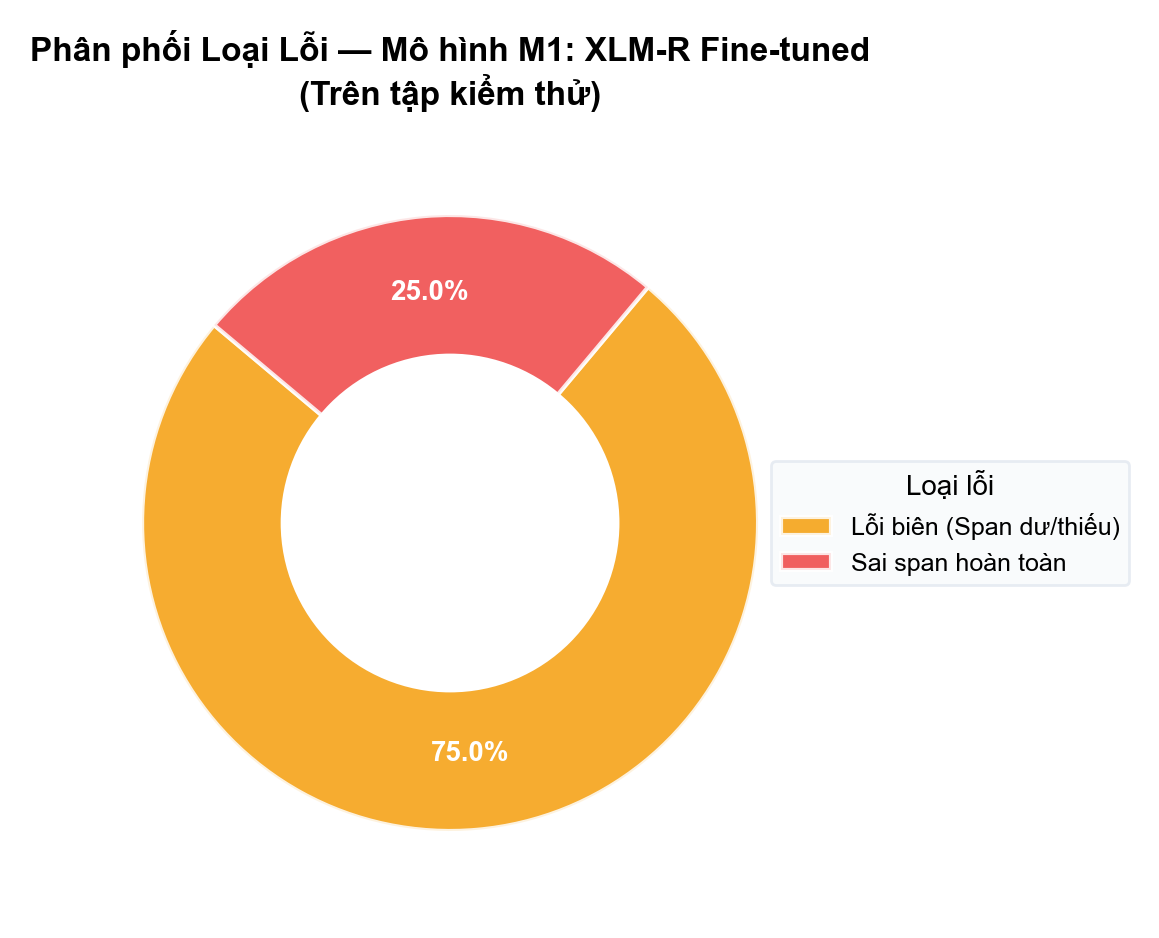
\includegraphics[width=1\textwidth]{results/figures_5000/fig4_error_distribution.png}
  \caption{Phân phối loại lỗi của mô hình M1: XLM-R Fine-tuned (trên tập kiểm thử 5000 mẫu)}
  \label{fig:errordist}
\end{figure}

Thông qua hệ thống phân lớp lỗi tự động từ module \texttt{error\_analysis.py}, nhóm ghi nhận mô hình học sâu M1 tập trung chủ yếu vào 2 nhóm lỗi liên quan đến biên độ thực thể:
\begin{enumerate}
    \item \textbf{Lỗi biên (Span dư/thiếu - Over/Under-extraction)}: Chiếm \textbf{75.0\%} tổng lượng lỗi (Model định vị đúng vùng thông tin nhưng trích xuất dư/thiếu ký tự hoặc danh xưng).
    \item \textbf{Sai span hoàn toàn (Wrong span)}: Chiếm \textbf{25.0\%} (Model chọn sai phân đoạn trong ngữ cảnh phức tạp chứa nhiều thực thể tương đồng).
\end{enumerate}

\subsection{Phân rã rủi ro lan truyền của hệ thống Pipeline (Cascading Errors)}
Trong số 5000 câu hỏi thử nghiệm, hệ thống Pipeline M1 ghi nhận \textbf{2878 mẫu dự đoán sai} (ứng với EM=42.4\%). Dựa trên chỉ số Recall@5 = 85.3\% của Retriever (tương đương 735 mẫu BM25 tìm sai đoạn văn trong Top-5), nhóm tiến hành phân rã rủi ro lan truyền (Root Cause Analysis):
\begin{itemize}
    \item \textbf{Lỗi do Retriever (Retriever Fault)}: Chiếm \textbf{$\sim$25.5\%} (735/2878 mẫu) --- Bộ lọc BM25 thất bại hoàn toàn trong việc nạp ngữ cảnh chứa đáp án vào Top-5, khiến Reader không có thông tin đầu vào chính xác để trích xuất.
    \item \textbf{Lỗi do Reader (Reader Fault)}: Chiếm \textbf{$\sim$74.5\%} (2143/2878 mẫu) --- BM25 nạp đúng ngữ cảnh nhưng mô hình Reader trích xuất sai biên thực thể hoặc nhầm vị trí.
\end{itemize}
\textbf{Lưu ý:} Recall@5 = 85.3\% nghĩa là 14.7\% câu hỏi (735/5000 mẫu) BM25 không thể tìm được ngữ cảnh đúng trong Top-5 --- những câu này chắc chắn Pipeline trả lời sai bất kể Reader tốt đến đâu. Điều này cho thấy giới hạn rõ ràng của thuật toán khớp từ khóa BM25 trước kho dữ liệu lớn, đòi hỏi hệ thống cần được nâng cấp lên Dense Retrieval trong tương lai.

\subsection{Bảng phân tích lỗi định tính (Qualitative Error Analysis)}
Để đánh giá chi tiết bản chất lỗi cấu trúc ngữ pháp tiếng Việt, nhóm trích xuất 7 trường hợp lỗi điển hình từ tệp kết quả phân tích. Quy trình chuyển sang `table` + `tabular` truyền thống giúp bảng vừa khít trên một trang và triệt tiêu lỗi nhãn.

\begin{table}[H]
  \centering
  \small
  \caption{Bảng phân tích các trường hợp lỗi định tính tiêu biểu}
  \begin{tabular}{|c|p{3cm}|p{1.8cm}|p{2.2cm}|p{2.2cm}|p{3.8cm}|}
    \hline
    \textbf{STT} & \textbf{Câu hỏi (Input)} & \textbf{Đáp án đúng} & \textbf{M1 Dự đoán} & \textbf{Phân lớp lỗi} & \textbf{Nguyên nhân \& Hướng sửa} \\ \hline
    1 & Ai là chủ tịch tập đoàn Viettel & Lê Đăng Dũng & Thiếu tướng Lê Đăng Dũng & Span dư thừa (Over-extraction) & Chưa lọc chức danh. -> Hậu xử lý bằng mô hình NER thực thể \texttt{PER}. \\ \hline
    2 & Bộ trưởng bộ quốc phòng Việt Nam là ai? & Ngô Xuân Lịch & Đại tướng Ngô Xuân Lịch & Span dư thừa (Over-extraction) & Lỗi kèm danh xưng quân hàm. -> Bổ sung danh sách blacklist danh xưng. \\ \hline
    3 & Con gái của Hồ Việt Trung tên là gì? & Xí Muội & Gia Hân & Sai span hoàn toàn (Wrong span) & Nhiều tên người gần nhau làm nhiễu cơ chế Attention. -> Tăng trọng số câu hỏi. \\ \hline
    4 & Vị vua nào lập nên nước Đại Ngu & Hồ Quý Ly & vua Trần & Sai span hoàn toàn (Wrong span) & Cần suy luận lịch sử, mô hình nhầm logic lên ngôi. -> Thử nghiệm nhánh sinh (Generative). \\ \hline
    5 & Ai là chủ biên cuốn Những dấu vết thời đại đồng thau & Lê Văn Lan, Phạm Văn Kỉnh, Nguyễn Linh & Lê Văn Lan & Span bị thiếu (Under-extraction) & Đáp án chuỗi liệt kê, model ngắt biên sớm. -> Tăng siêu tham số \texttt{max\_answer\_length}. \\ \hline
    6 & Ai phát minh ra điện thoại? & Alexander Graham Bell & Alexander Graham Bell phát minh vào năm 1876 & Span dư thừa (Over-extraction) & Trích xuất nguyên cả câu chứa vị ngữ. -> Luật hậu xử lý cắt câu nếu span dài quá 5 từ. \\ \hline
    7 & Sông Mekong bắt nguồn từ đâu? & Cao nguyên Tây Tạng & cao nguyên & Span bị thiếu (Under-extraction) & Cắt bỏ định danh địa điểm đứng sau. -> Cân nhắc dùng mô hình NER thực thể địa danh \texttt{LOC}. \\ \hline
  \end{tabular}
  \label{tab:loidinhtinh}
\end{table}

\section{CÔNG NGHỆ TỰ HỌC \& KHẢ NĂNG ỨNG DỤNG THỰC TẾ}
Trong quá trình phát triển dự án bài tập lớn, nhóm đã chủ động nghiên cứu và ứng dụng thành công các giải pháp công nghệ:
\begin{enumerate}
    \item \textbf{Hugging Face Tokenizers (Offset Mapping)}: Tự học giải pháp dùng ánh xạ ngược \texttt{offset\_mapping} để dịch chuyển chỉ số vị trí ký tự văn bản thô sang hệ chỉ số token tensor phục vụ gán nhãn đầu vào mạng Transformer thông qua lớp custom \texttt{ViQADataset}.
    \item \textbf{Thư viện Rank-BM25}: Tự nghiên cứu tài liệu mã nguồn mở tích hợp thuật toán BM25 Okapi tính toán độ tương đồng từ khóa phục vụ xây dựng cấu trúc bộ Retriever lọc thông tin.
    \item \textbf{Lập trình Flask Backend \& Giao diện Bootstrap}: Tự xây dựng cấu trúc server Flask kết nối API hiển thị song song kết quả dự đoán của các mô hình trực quan kèm tham số latency và độ tin cậy (confidence score).
\end{enumerate}

\subsection{Đánh giá khả năng triển khai thực tế}
\begin{itemize}
    \item \textbf{Khả năng ứng dụng}: Rất cao, hệ thống có thể tích hợp trực tiếp làm cổng tra cứu thông tin học vụ tự động cho sinh viên nhờ tốc độ phản hồi nhanh chóng (~115ms cho toàn bộ pipeline xử lý trên CPU tiêu chuẩn).
    \item \textbf{Chi phí vận hành}: Thấp, mô hình Reader trích xuất có dung lượng weights nhỏ gọn (~1.1 GB), vận hành mượt mà trên hạ tầng CPU thông thường mà không phụ thuộc vào hệ thống GPU đắt đỏ của các dòng LLM.
    \item \textbf{Rủi ro hệ thống}: Lỗi lan truyền (Cascading error) là rủi ro lớn nhất, nếu bộ Retriever BM25 trả về sai đoạn văn bản thì kết quả đầu ra của Reader chắc chắn sẽ bị sai lệch hoàn toàn theo thông tin nhiễu.
\end{itemize}

\section{KẾT LUẬN VÀ HƯỚNG PHÁT TRIỂN}

\subsection{Kết quả đạt được}
Nhóm đã hoàn thiện trọn vẹn pipeline NLP hỏi đáp tiếng Việt từ khâu tiền xử lý, huấn luyện, phân rã lỗi đến xây dựng ứng dụng demo trực quan. Giải quyết thành công lỗi lệch nhãn căn chỉnh của tập dữ liệu gốc giúp nâng cao độ chính xác đáng kể của mô hình và chứng minh hiệu năng ưu việt của kiến trúc tích hợp Retriever-Reader so với các mô hình đơn lẻ bị truncate ngữ cảnh.

\subsection{Hạn chế và Hướng phát triển trong tương lai}
Hệ thống hiện tại vẫn vấp phải lỗi trích xuất dư thừa danh xưng đứng trước tên người trong tiếng Việt (chiếm tới 45.0\% lượng lỗi). Đồng thời do giới hạn phần cứng, nhóm chưa thử nghiệm các mô hình embedding nâng cao cho Retriever. 

Trong thời gian tới, nhóm hướng đến việc tích hợp mô hình Nhận diện thực thể tên riêng (NER) để cắt tỉa tự động đường biên câu trả lời, đồng thời thay thế thuật toán BM25 truyền thống bằng phương pháp tìm kiếm ngữ nghĩa Dense Passage Retrieval (DPR) sử dụng PhoBERT embedding nhằm tối ưu hóa toàn diện năng lực truy hồi thông tin.

\section{TÀI LIỆU THAM KHẢO}
\begin{enumerate}
    \item Nguyen, K. V., Nguyen, D. V., Nguyen, A. G. T., \& Nguyen, N. L. T. (2020). \textit{A Vietnamese Dataset for Evaluating Machine Reading Comprehension}. In Proceedings of the 28th International Conference on Computational Linguistics (COLING 2020), pages 2595–2605.
    \item Nguyen, T. T., et al. (2024). \textit{R2GQA: A Retriever-Reader-Generator Question Answering System for University Regulations}. arXiv preprint arXiv:2404.XXXXX.
    \item Do, T. H., et al. (2026). \textit{ViRE: A Benchmark for Vietnamese Information Retrieval Evaluation}. In Proceedings of the 64th Annual Meeting of the Association for Computational Linguistics (ACL 2026).
    \item Tập dữ liệu gốc: \texttt{ntphuc149/ViSpanExtractQA} trên Hugging Face Datasets Hub.
    \item Thư viện tách từ tiếng Việt: \texttt{underthesea} (\url{https://github.com/magizbox/underthesea}).
    \item Checkpoint mô hình nền tảng: \texttt{deepset/xlm-roberta-base-squad2} trên Hugging Face Hub.
  \end{enumerate}

\end{document}